\documentclass[a4j,twocolumn]{ltjarticle}

%ページ設定
\setlength{\topmargin}{-10mm}
\setlength{\oddsidemargin}{-5mm}
\setlength{\evensidemargin}{-5mm}

\setlength{\textheight}{230mm}
\setlength{\textwidth}{170mm}
\setlength{\columnsep}{10mm}%コラムとコラムの間.よってコラムの横幅は(texwidth-columnsep)/2
\setlength{\footskip}{15mm}
%パッケージ
\usepackage{graphicx,color}
\usepackage{bm}
\usepackage{amsmath}
\usepackage{amsfonts}

%数学関数
\newcommand{\B}[1]{\bm #1} 
\newcommand{\s}[2]{{#1}\cdot{#2}} 
\newcommand{\R}{\mathbb{R}}
\newcommand{\M}{\mathbb{M}}
\newcommand{\df}[2]{\displaystyle{\frac{#1}{#2}}}
\newcommand{\qed}{
\begin{flushright}
\vspace{-8mm}
$\Box$
\end{flushright}
}

%ミニセクション
\newcommand{\minisection}[2]{\flushleft{\bf (#1)#2}\\ \ \ \ }

%図,表の名前変更
\renewcommand{\figurename}{Fig.}
\renewcommand{\tablename}{Tab.}

% refの拡張
\newcommand{\reffig}[1]{\figurename \ref{#1}}
\newcommand{\refeq}[1]{式(\ref{#1})}
\newcommand{\reftab}[1]{\tablename \ref{#1}}

% 図
\newcommand{\includefigure}[3]{
\begin{center}
\includegraphics[width=80mm]{#1}
\caption{#2}
\label{#3}
\end{center}
}
% 図 widthを変更したいときはこっち
\newcommand{\includefigurewidth}[4]{
\begin{center}
\includegraphics[width=#2]{#1}
\caption{#3}
\label{#4}
\end{center}
}

\usepackage{setspace} % setspaceパッケージのインクルード
\usepackage{enumitem}
\usepackage{graphicx}
%「Weekly Report」 
\newcommand{\Weekly}[5]{
\twocolumn[
 \begin{center}
  \bf
 第 #1 回 Weekly Report\\
 \huge
深層学習を用いた動画像からの危険認知手法のための基礎的研究\\

 \end{center}
 \begin{flushright}
  #2 月\ \ \  #3 日 \ \ \ #4 \\\
  #5
 \end{flushright}
]
}
%\setstretch{0.5} % ページ全体の行間を設定

\begin{document}

\Weekly{7}{6}{30}{(火)}{\ 小松 大起}
\section{本実験の目的}
危険認知手法実現のために動画像を用いた深層学習によって次フレームの画像を用いた深層学習によって次フレームの画像を予測し生成を行い,その画像と実際の画像を比べる.
\section{PredNet}
PredNet は Deep Recurrent Convolutional Neural Network  の 1 種で 神経科学の概念である Predictive Coding を組み込んで作られたモデルである. 2016 年に William Lotter, Gabriel Kreiman, David Cox の 3 氏によって公開された.

\subsection{PredNet の層構造}
PredNet の各層には 4 つの素子が存在しておりそれぞれ、Target, Representation, Prediction, Errorと呼ぶ.
Target は下層からの出力である誤差信号をエンコード,符号化する.
Representation は Recurrent unitで,上層からの出力,側方からの誤差信号, 1 ステップ前の自分の出力を受け取る.
Representation unit は Target の予測をする Prediction unit に投射し,入力の予測が出力される.
Error は Prediction と Target の誤差であり, Error は上層に送られる.
この Error が小さくなるように学習を進めていく.
また,層構造の例を図 2 に示す.

 \begin{figure}[hb]
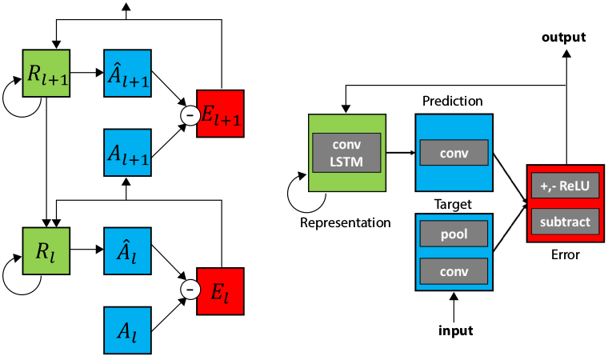
\includegraphics[scale=0.4]{prednet.png}
 \caption{PredNet の層構造の例}
\end{figure}
%%%%%%%%%%
\begin{figure}[hb]
\includegraphics[scale=0.4]{DeepPrednet_formula.png}
 \caption{PredNet の更新式}
\end{figure}
更新式は(1)から(4)のように表される.

\section{使用した動画像}
\subsection{KITTI}
ドイツの都市環境を運転している車の屋根に取り付けられたカメラによってキャプチャされたデータセットである.City, Residential, Road のカテゴリに分かれており,それぞれ都市街,住宅地,高速道路というようなシーン分けがされている.それぞれのカテゴリには City には 28 シーン, Residential には 21 シーン, Road には 12 シーン存在している.合計 61 のシーンがあるが,それぞれのカテゴリから 10 フレームがテストデータとしてサンプリングされ, 57 シーンが訓練に用いられ, 4シーンが検証に用いられる.

\section{オートエンコーダ}
オートエンコーダの目的は次元削減を行うこと.
\section{先週までの作業}
\begin{itemize}
          \item PredNet について
          \item 授業課題
          \item PredNet の出力を得られた 図に示す。1 フレーム先の画像を予測するように訓練されている.
\begin{figure}[hb]
\begin{center}
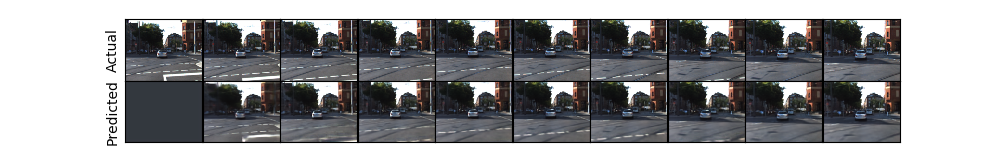
\includegraphics[scale=0.8]{plot_1.png}
\caption{PredNet の出力結果}
\end{center}
\end{figure}

\end{itemize}

\section{今週の作業}
\begin{itemize}       
         \item prednet 数式理解
         \item オートエンコーダを prednet に組み込む
         \item 金曜日に企業説明会に参加する
\end{itemize}

\section{来週以降の作業}
\begin{itemize}
         \item 
\end{itemize}




\end{document}
